\documentclass{article}
\usepackage{graphicx}
\usepackage[utf8]{inputenc}
\usepackage{hyperref}
\usepackage[brazil]{babel}

\title{especificacao-requisitos}
\author{andrefilipedasilvafernandes }
\date{May 2022}

\hypersetup{
    colorlinks=true,
    linkcolor=blue,
    filecolor=magenta,      
    urlcolor=cyan
    }
    
\begin{document}

\begin{titlepage}
\begin{center}
    {\large Universidade Federal de Santa Catarina - UFSC}\\[0.2cm]
    {\large Departamento de Informática e Estatística - INE}\\[0.2cm]
    {\large Curso de Ciências da Computação}\\[0.2cm]
    {\large INE5417 - Engenharia de Software I}\\[5.1cm]
    {\bf \huge Especificação de Requisitos: \\ Jogo Chaturanga}\\[5.1cm]
\end{center}

\begin{flushright}
    {\bf \large  Alunos:} \\
        André Filipe da Silva Fernandes \\
        Gabriel Holstein Meireles \\
        Eduardo Vicente Petry \\
    [0.7cm]
        
    {\bf \large Professor:}\\
        Ricardo Pereira e Silva \\
    [0.7cm]
\end{flushright}

\begin{center}
    {\large Florianópolis}\\[0.2cm]
    {\large 2022}
\end{center}

\end{titlepage} %término da "capa"
\pagebreak

\section{Introdução}
\subsection{Objetivo do Desenvolvimento}
    Desenvolvimento de um software para computador que permita a disputa local entre dois jogadores em uma partida de Chaturanga, um antigo jogo indiano.

\subsection{Referências}
    \url{https://www.chessvariants.com/historic.dir/chaturanga.html} \\
    \url{https://en.wikipedia.org/wiki/Chaturanga} \\
    
\section{Visão Geral do Sistema}
\subsection{Arquitetura do Programa}
    Programa orientado a objetos escrito na linguagem Python.
    
\subsection{Descrição do Jogo}
    Chaturanga é um jogo composto por dois jogadores, um tabuleiro 8x8 e 16 peças para cada jogador.
    As 16 peças compõem um exército e se dividem em oito Padati, dois Ratha, dois Ashwa, dois Gaja, um Mitri e um Raja.
    
    A distribuição do exército no tabuleiro para o início da partida se dá como na imagem \ref{figura:initial_board}.
    
    \begin{figure}[h]
    \centering
    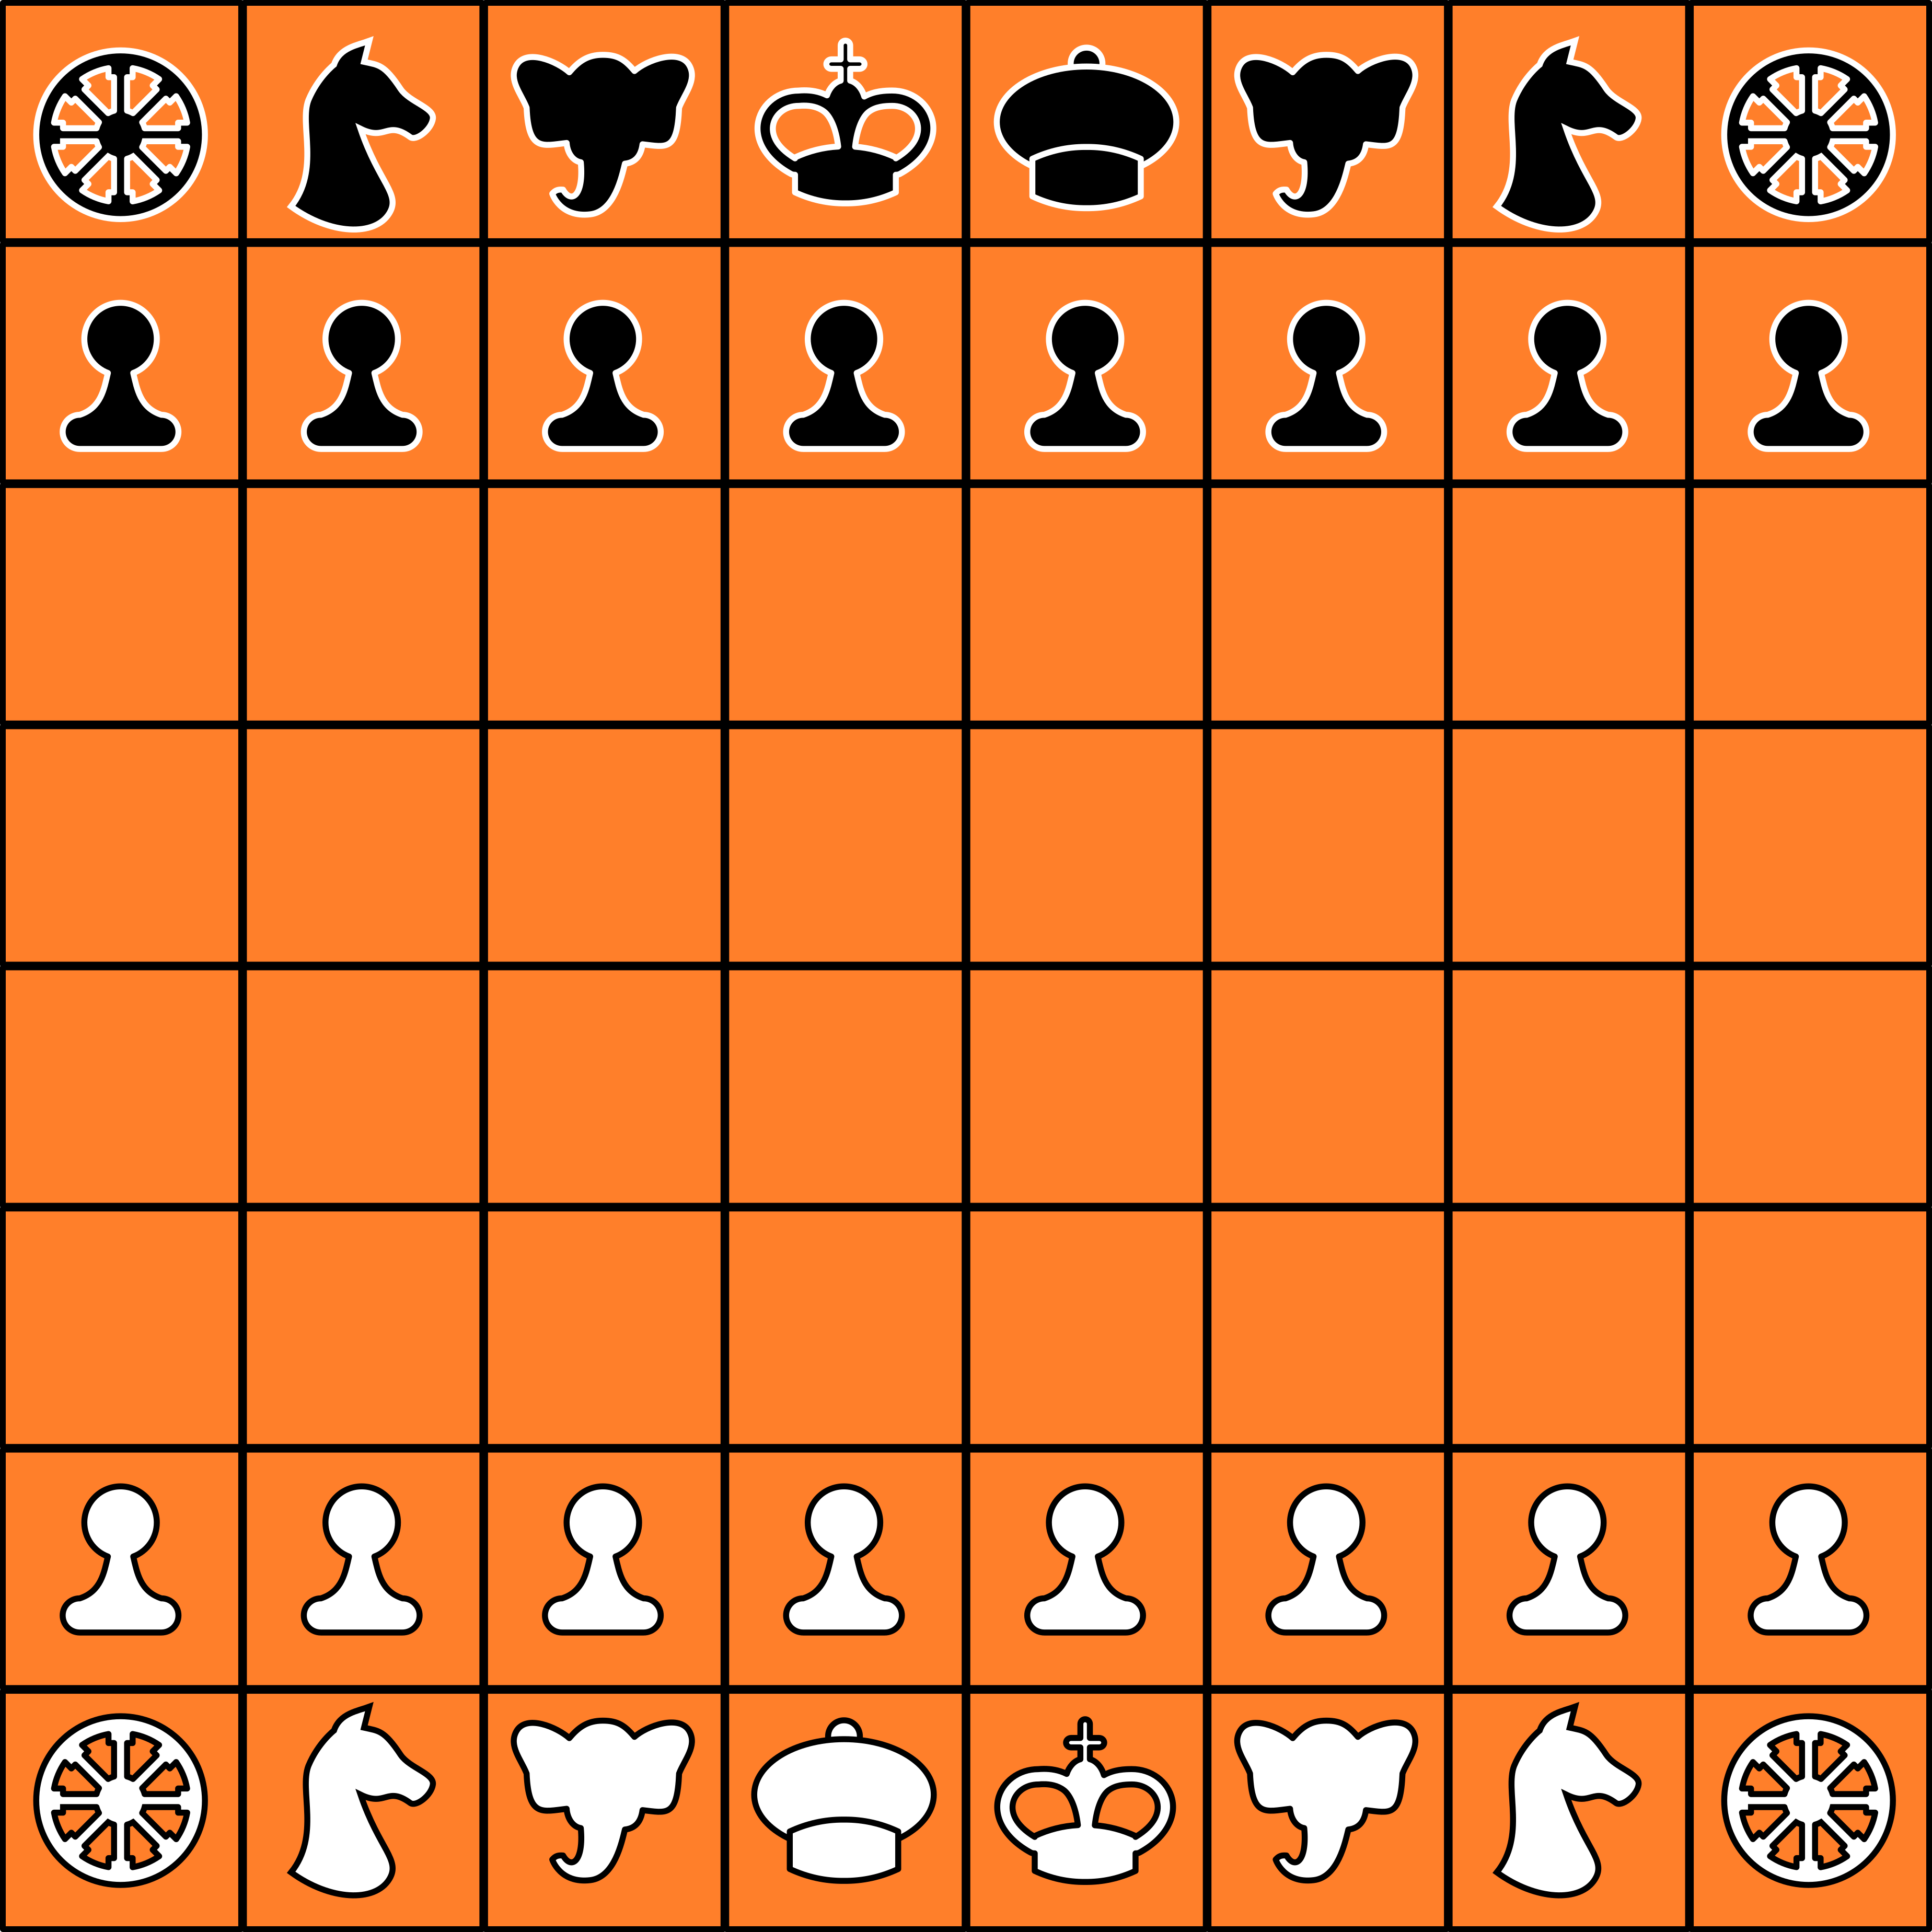
\includegraphics[width=7cm]{imgs/initial_board.png}
    \caption{Configuração Inicial do Tabuleiro}
    \label{figura:initial_board}
    \end{figure}

    O jogador com as peças brancas deve iniciar a partida, então, os turnos alternam entre os dois jogadores. O objetivo do jogo é capturar o Raja inimigo ou aniquilar o exército adversário.

    A cada turno, o jogador escolhe uma peça que controla e a move para alguma casa vazia ou captura uma peça adversária.
    
    As regras de movimento para cada peça são as seguintes:

    \begin{itemize}
        \item Padati (Soldado): anda uma casa diretamente para frente ou, no caso de existir uma peça inimiga na sua diagonal direta, captura uma peça inimiga em sua diagonal direta, como na figura \ref{figura:padati_moves}.
        
        \item Ratha (Carruagem): anda em movimento ortogonal ao tabuleiro, ou seja, tanto para frente/trás quanto para esquerda/direita e se move quantas casas forem desejadas como na figura \ref{figura:ratha_moves}.
        
        \item Ashwa (Cavalo): anda imediatamente na diagonal oposta de um retângulo 3x2 e ignora qualquer peça que exista no caminho como na figura \ref{figura:ashwa_moves}.
        
        \item Gaja (Elefante): anda duas casas em uma diagonal adjacente e ignora qualquer peça que exista no caminho, ou uma casa diretamente para frente como na figura \ref{figura:gaja_moves}.
        
        \item Mitri (Ministro): anda uma casa em uma diagonal adjacente como na figura \ref{figura:mitri_moves}.
        
        \item Raja (Rei): anda uma casa em qualquer direção adjacente como na figura \ref{figura:raja_moves}.
        
    \end{itemize}
    
    Nota-se que no caso das peças que tem movimento de várias casas, elas param ao colidir com uma peça aliada ou ao capturar uma inimiga a não ser que seja especificado que ignoram outras peças. Em caso de movimento que resulta em captura, a peça que fez o movimento passa a ocupar a casa previamente pertencente a capturada.

    No caso especificamente do Padati, há a possibilidade de promoção para virar um Mitri. Para isso, é necessário que a peça encoste na borda do tabuleiro pertencente ao exército do adversário.
    
    \begin{figure}[h]
    \centering
    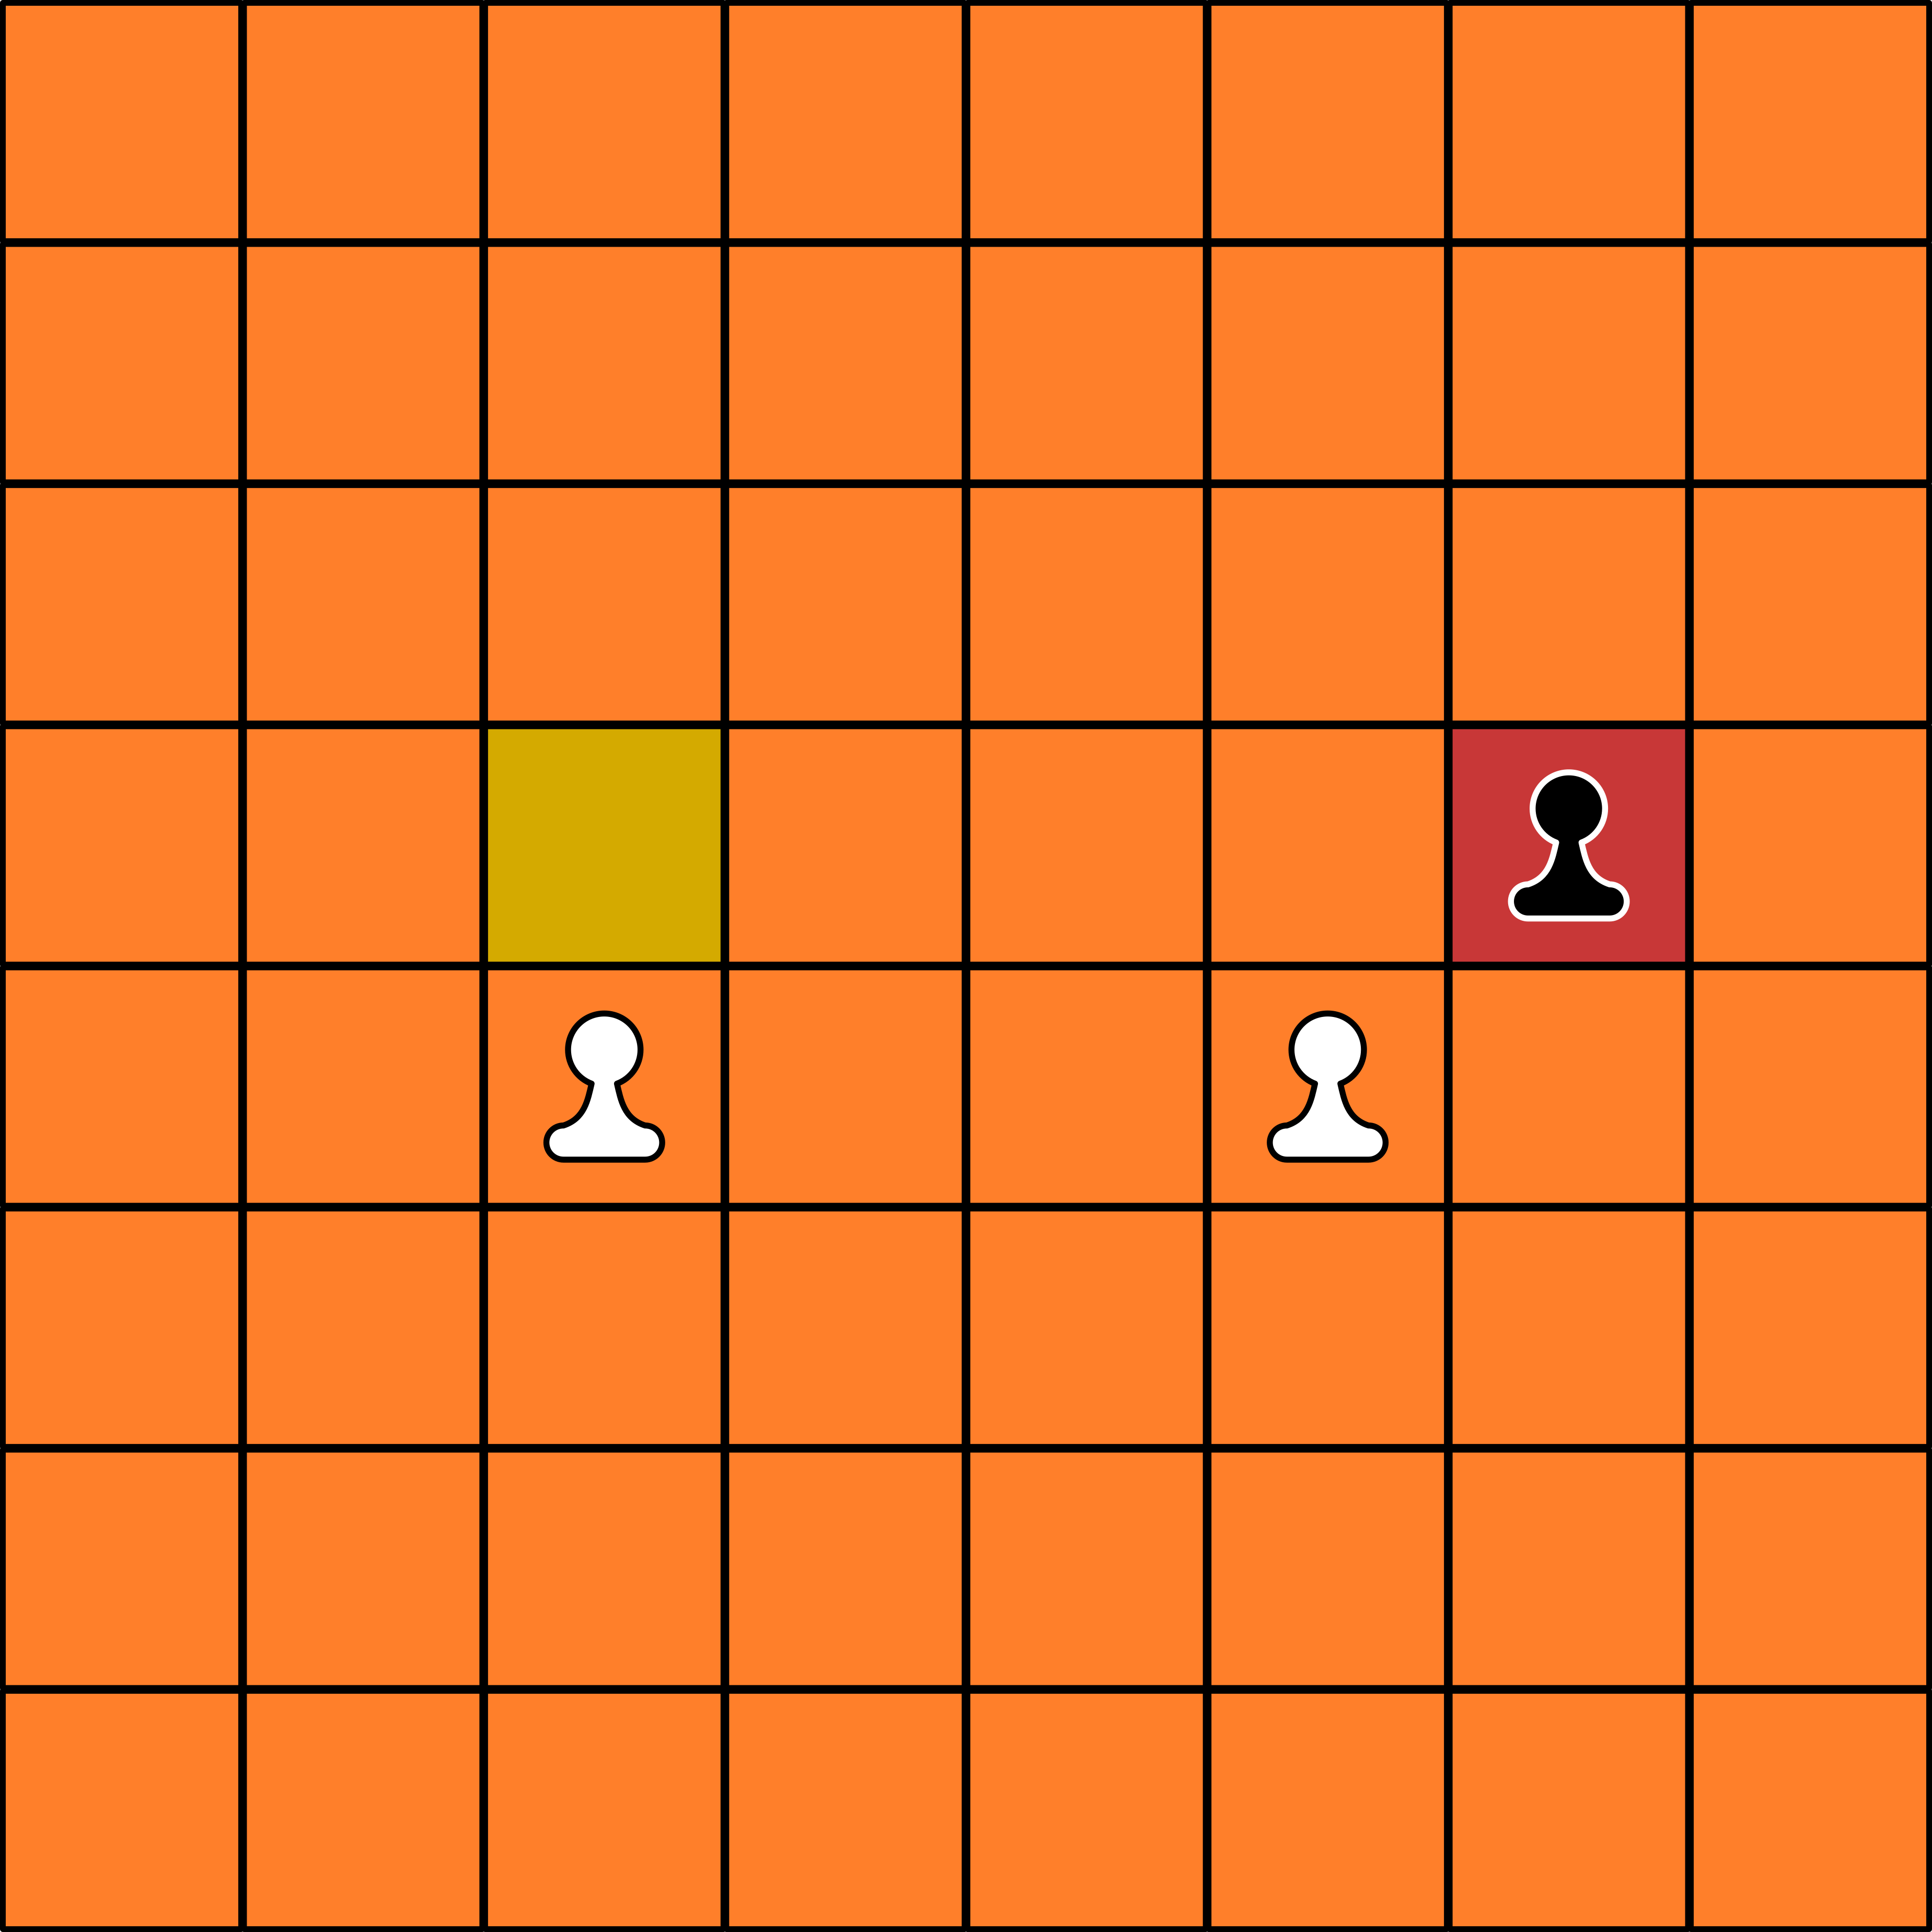
\includegraphics[width=5cm]{imgs/padati_moves.png}
    \caption{Movimentação do Padati (Soldado)}
    \label{figura:padati_moves}
    \end{figure}
    
    \begin{figure}[h]
    \centering
    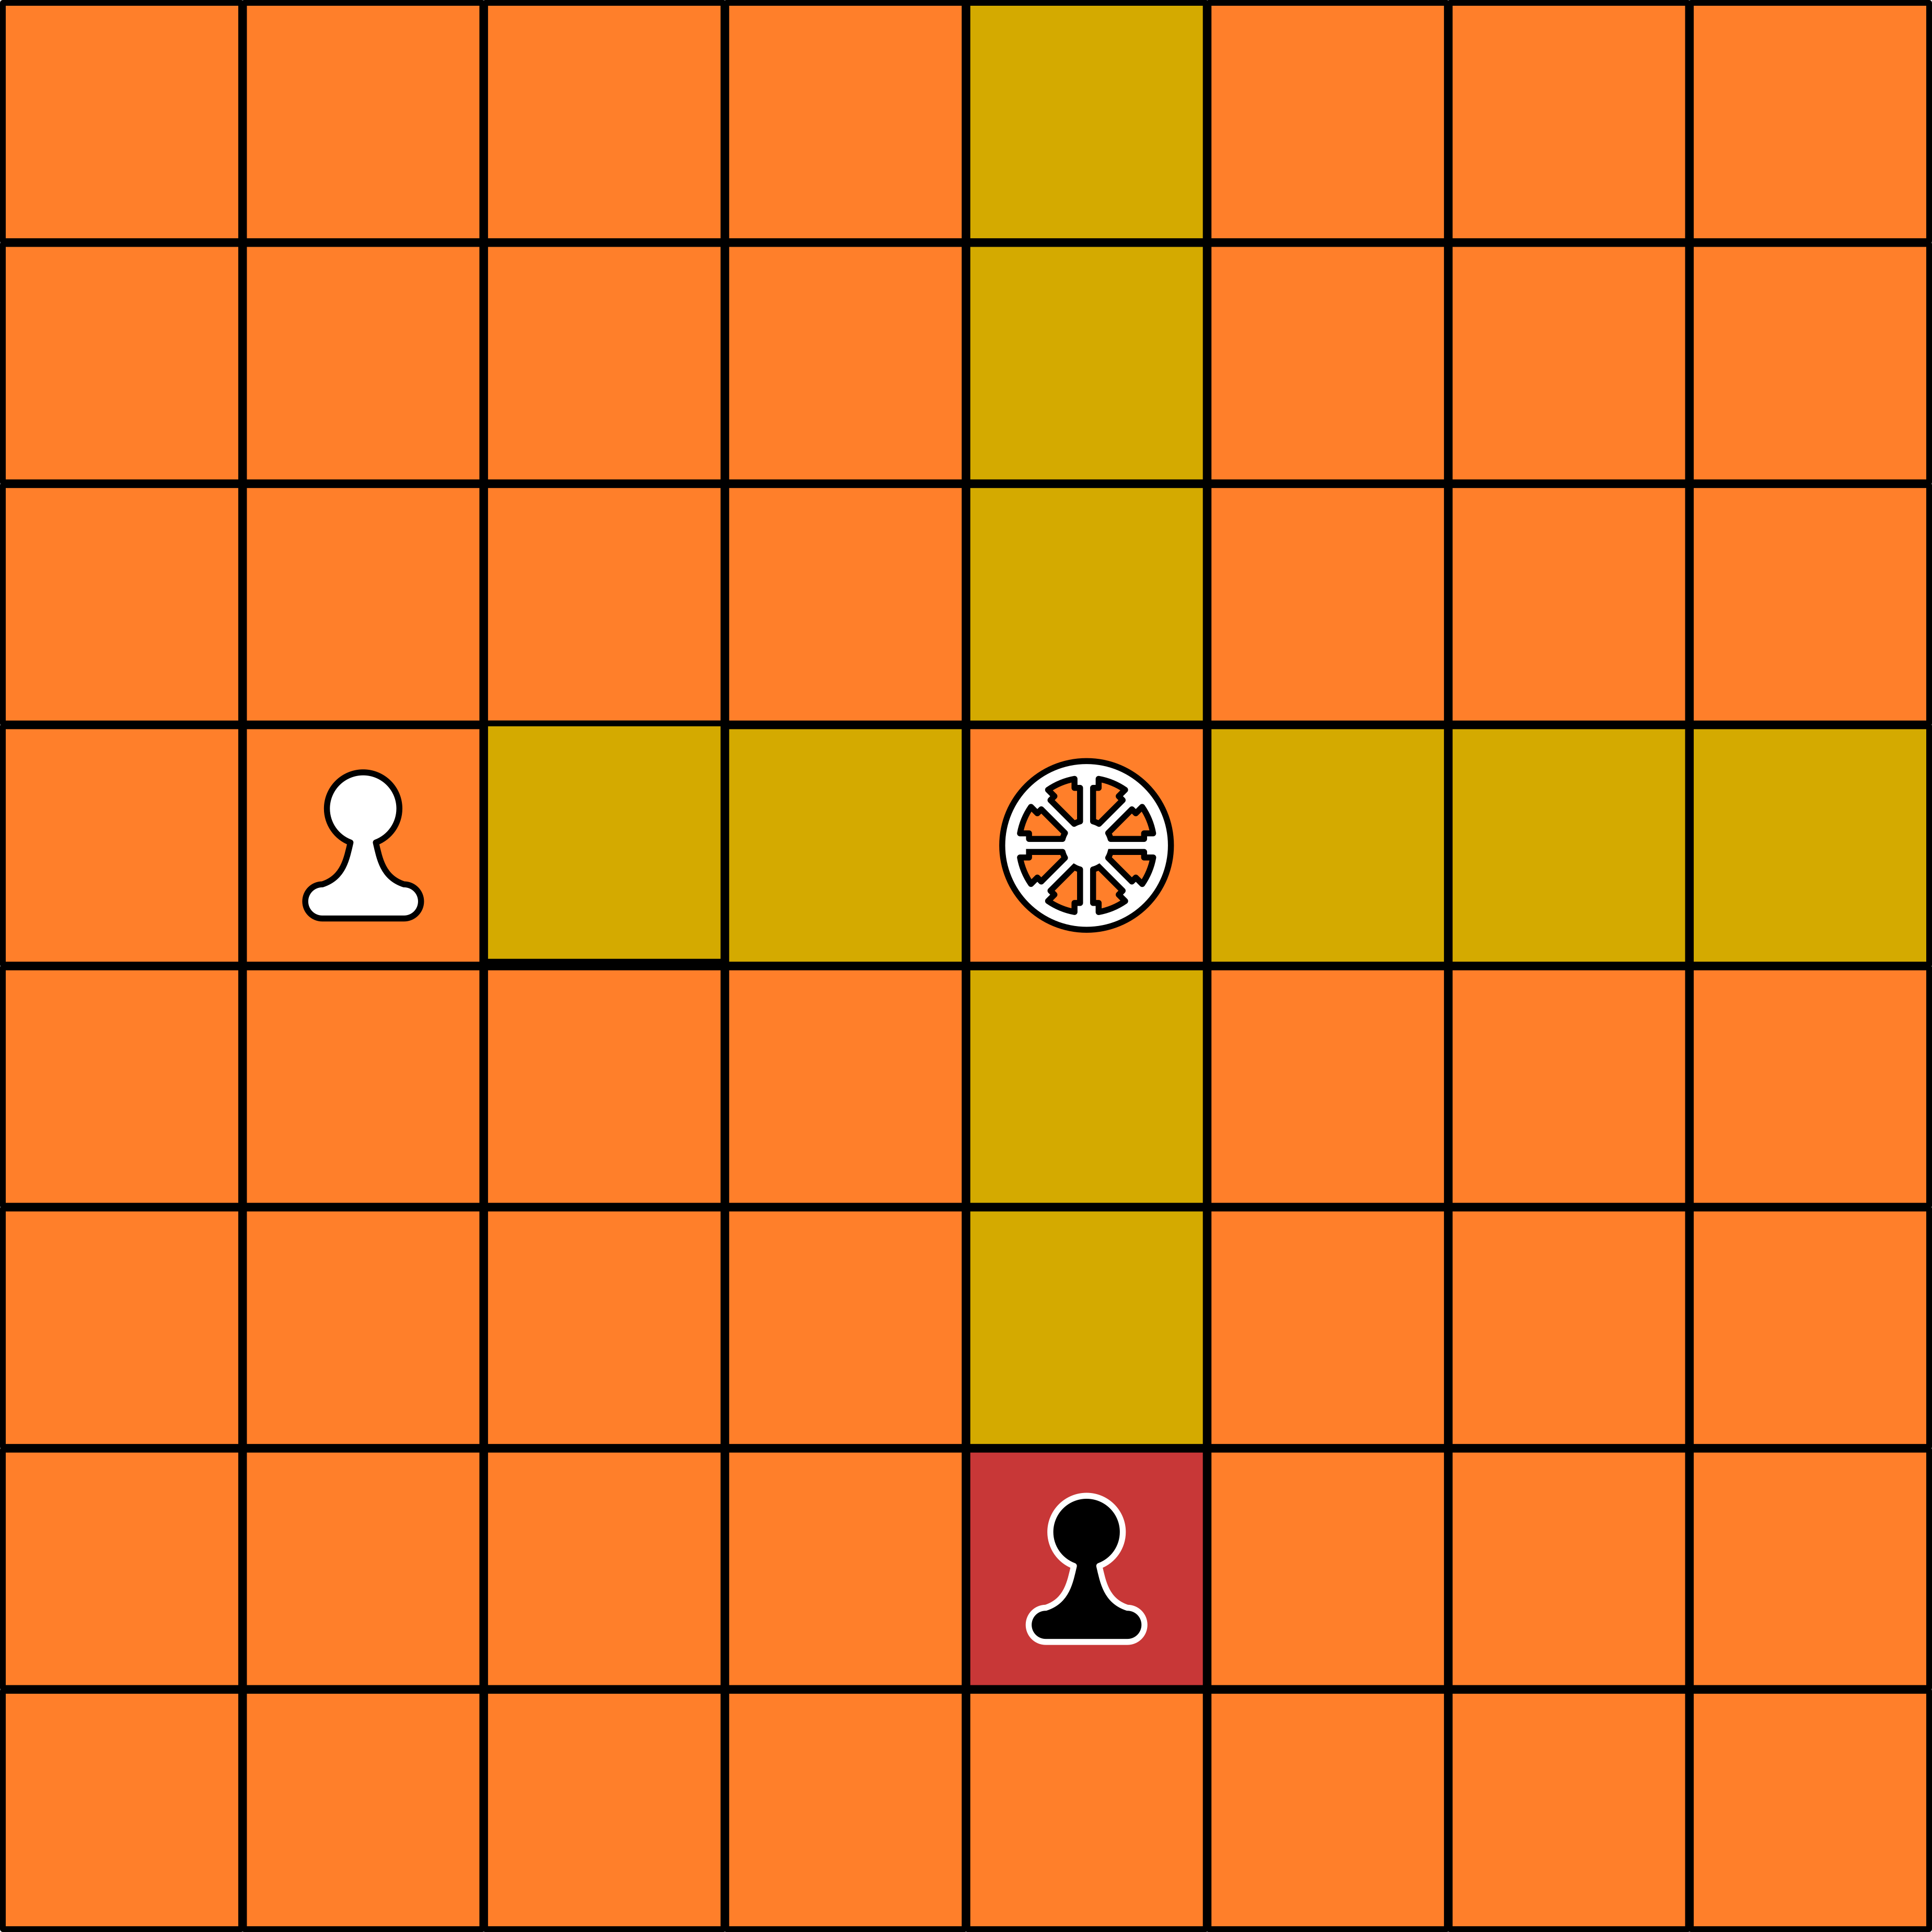
\includegraphics[width=5cm]{imgs/ratha_moves.png}
    \caption{Movimentação do Ratha (Carruagem)}
    \label{figura:ratha_moves}
    \end{figure}

    \begin{figure}[h]
    \centering
    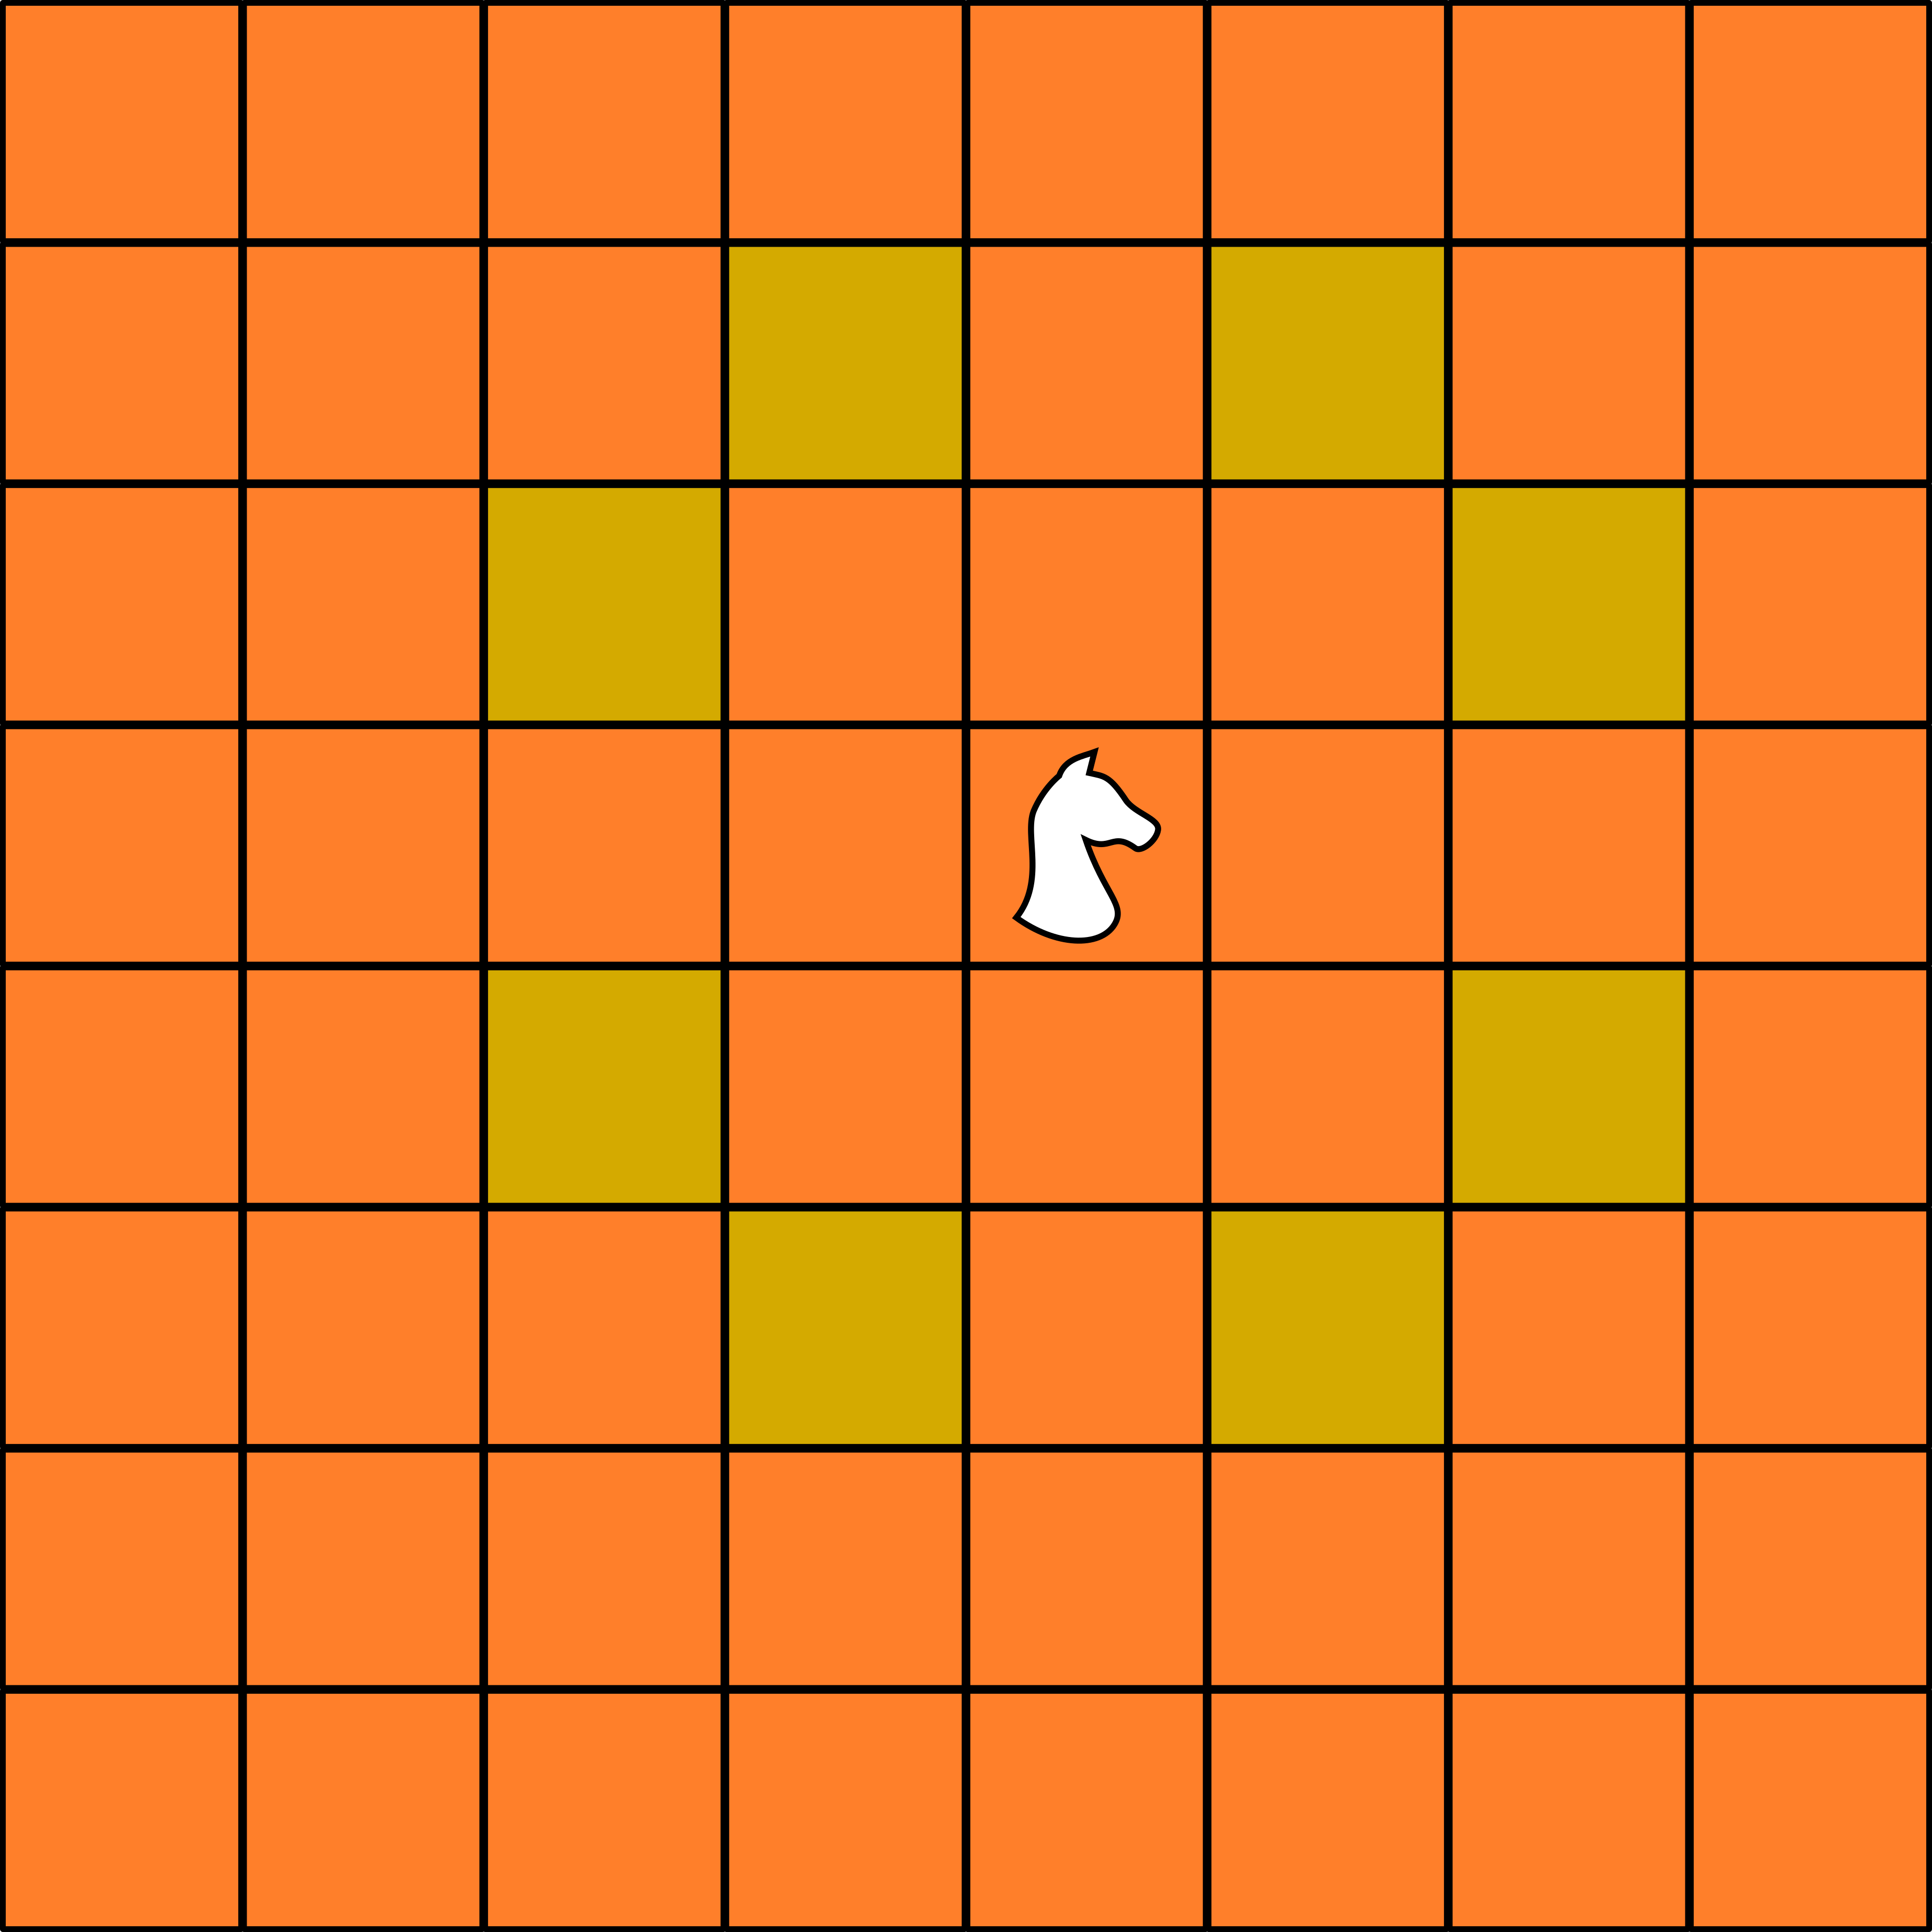
\includegraphics[width=5cm]{imgs/ashwa_moves.png}
    \caption{Movimentação do Ashwa (Cavalo)}
    \label{figura:ashwa_moves}
    \end{figure}
    
    \begin{figure}[h]
    \centering
    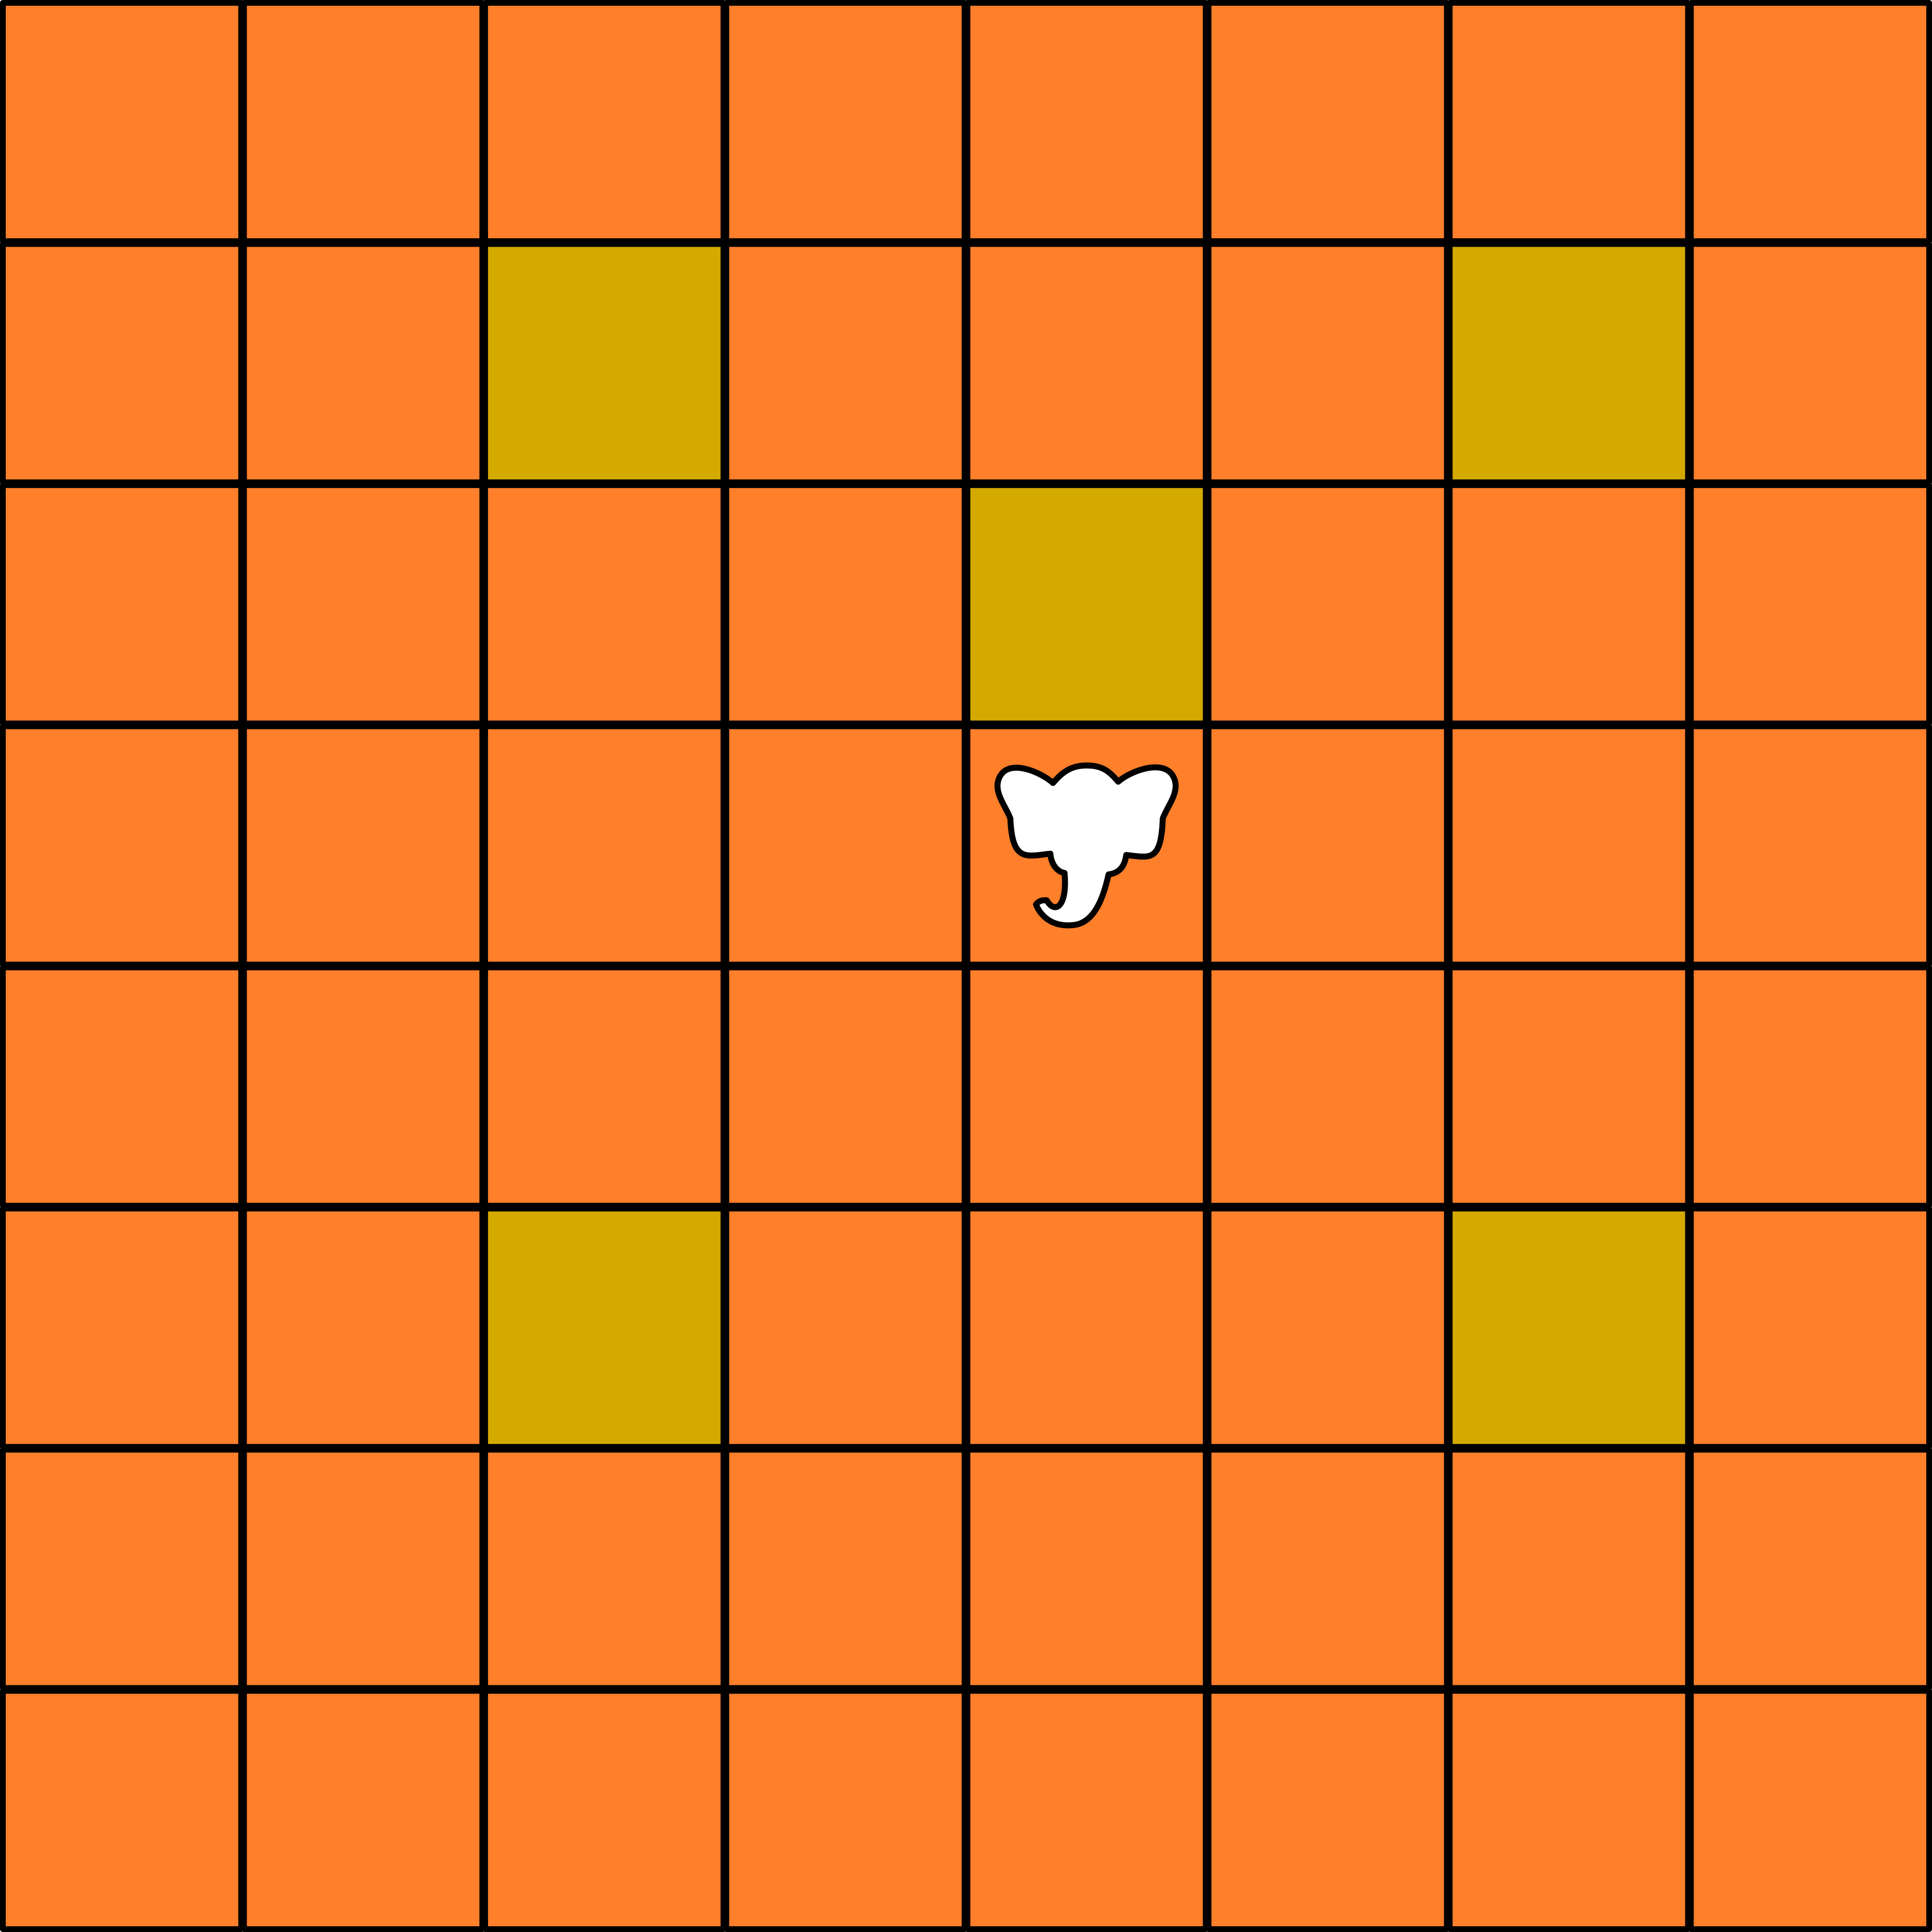
\includegraphics[width=5cm]{imgs/gaja_moves.png}
    \caption{Movimentação do Gaja (Elefante)}
    \label{figura:gaja_moves}
    \end{figure}
    
    \begin{figure}[h]
    \centering
    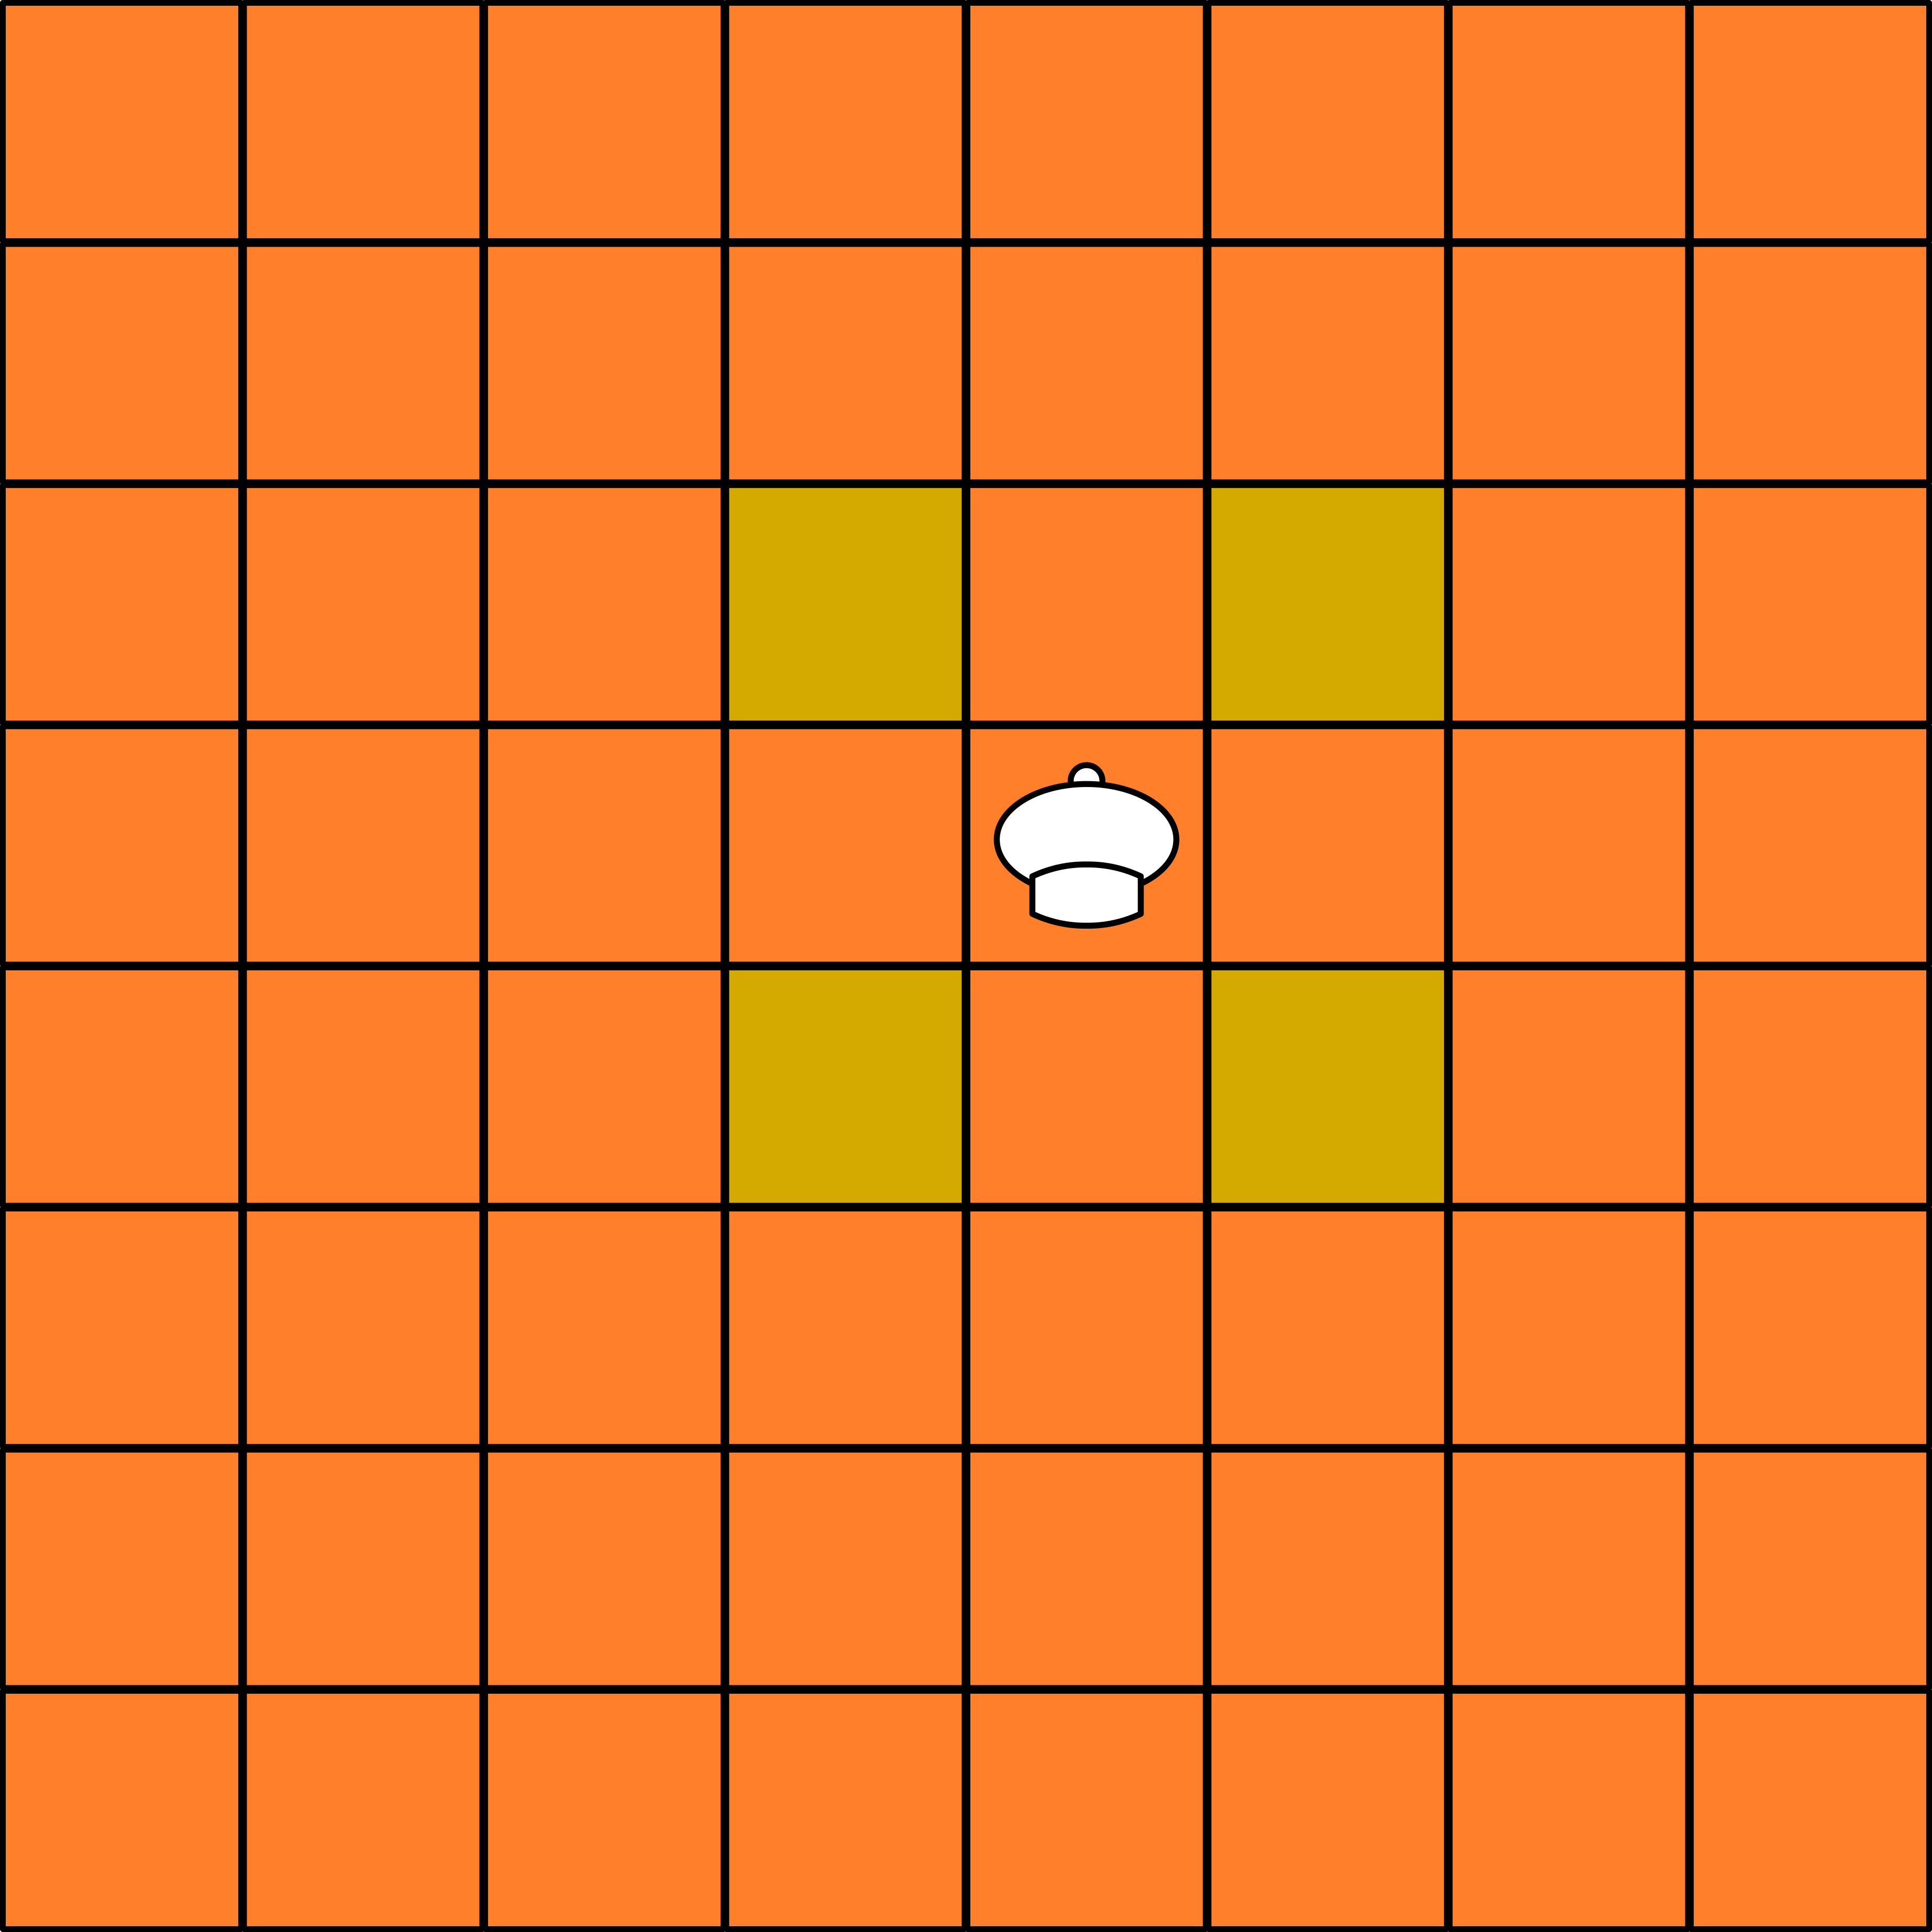
\includegraphics[width=5cm]{imgs/mitri_moves.png}
    \caption{Movimentação do Mitri (Ministri)}
    \label{figura:mitri_moves}
    \end{figure}

    \begin{figure}[h]
    \centering
    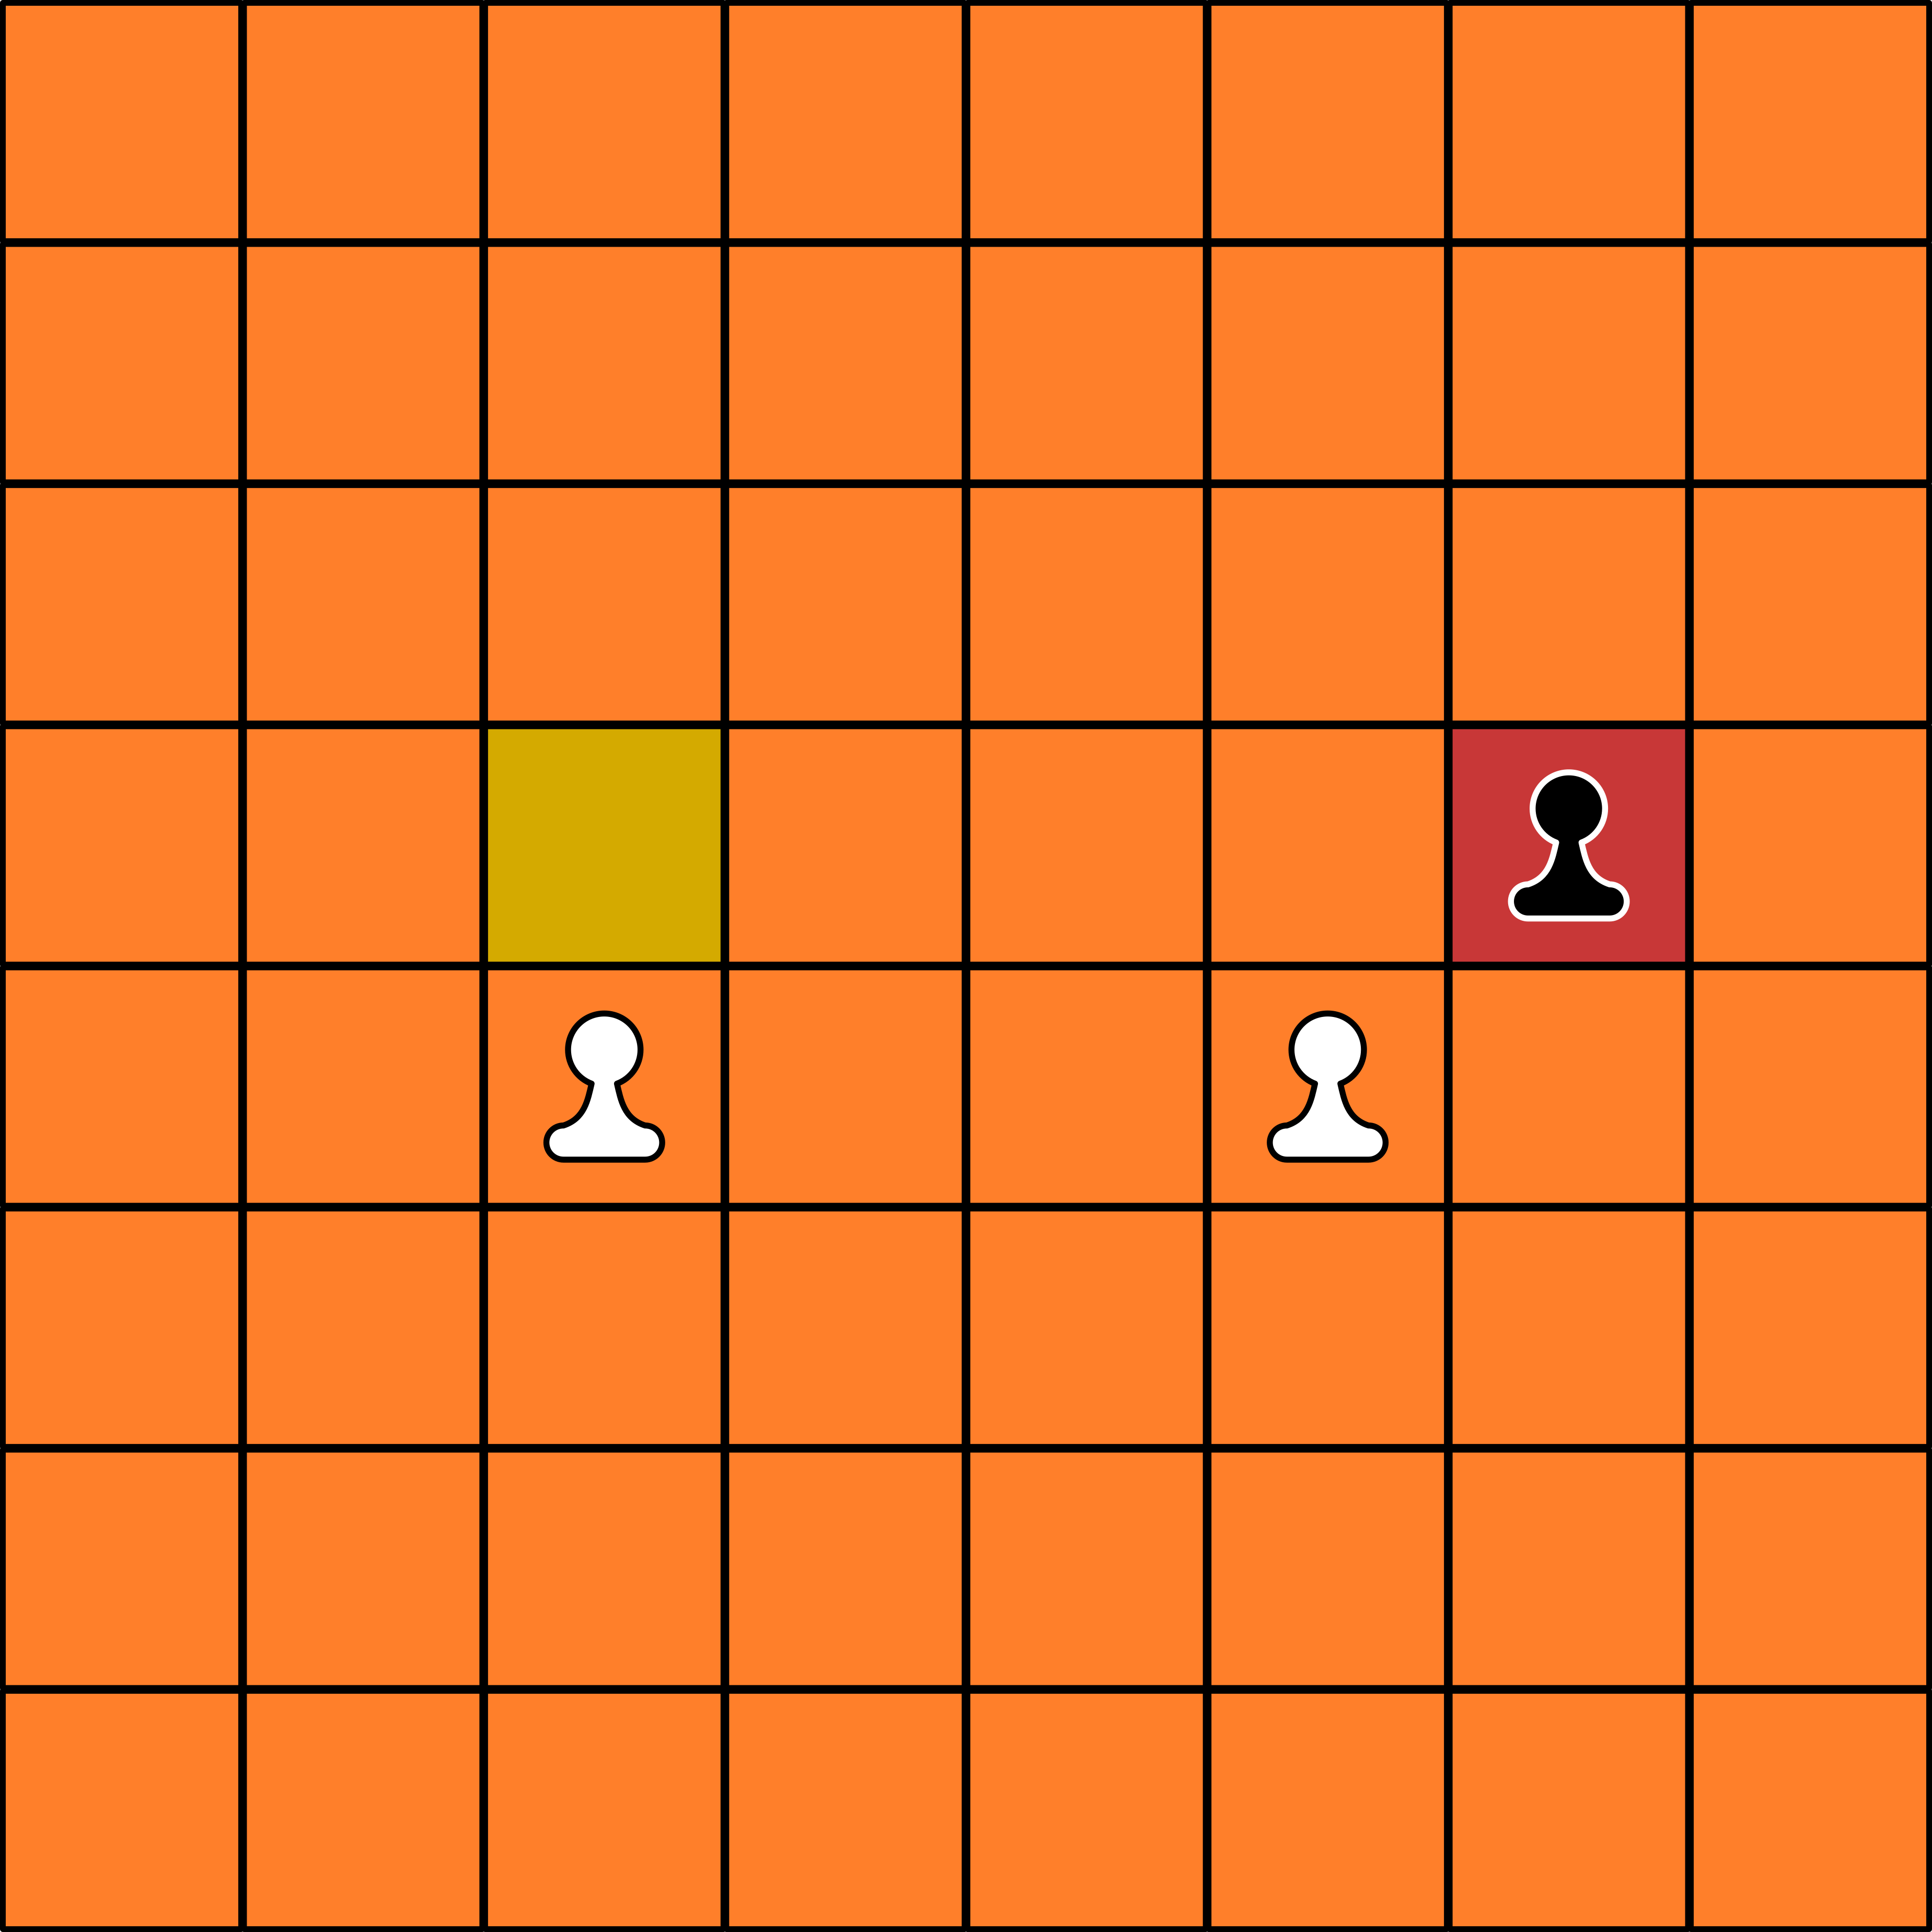
\includegraphics[width=5cm]{imgs/padati_moves.png}
    \caption{Movimentação do Raja (Rei)}
    \label{figura:raja_moves}
    \end{figure}

\subsection{Premissas de Desenvolvimento}
    \begin{itemize}
        \item O programa será desenvolvido com a linguagem de programação Python 3 sob o paradigma de Orientação a Objetos.
        
        \item O programa deverá apresentar uma interface bidimensional, onde cada jogador irá interagir com o uso do mouse.
        
        \item O jogo será implementado em português.
        
    \end{itemize}
    
\section{Requisitos de Software}

\subsection{Requisitos Funcionais}

\subsection{Requisitos Não Funcionais}

    Requisitos Não Funcional 1 - Especificação de Projeto: 
    Além do código python deve ser produzida especificação de projetos baseada em UML2, através da ferramenta Visual Paradigm.
    
    Requisitos Não Funcional 2 - Interface Gráfica:
    O programa deve implementar a interface gráfica utilizando as bibliotecas Tkinter ou Pyqt5.

\subsection{Esboço da Interface}

    

    
\end{document}
